\documentclass[11pt, a4paper]{article}

\usepackage[utf8]{inputenc}
\usepackage{amsmath, amssymb, amsthm}
\usepackage{geometry}
\usepackage{tikz}
\usetikzlibrary{positioning, arrows.meta, matrix, shapes.geometric, calc, shadows}
\usepackage{hyperref}

\geometry{margin=1in}

% Theorem environments
\newtheorem{definition}{Definition}
\newtheorem{theorem}{Theorem}
\newtheorem{remark}{Remark}

% Macros
\newcommand{\F}{\mathbb{F}}
\newcommand{\C}{\mathcal{C}}
\newcommand{\X}{\mathcal{X}}
\newcommand{\cL}{\mathcal{L}}

\title{\textbf{Lecture Notes: Structural Viewpoints of Linear Block Codes}}
\author{Coding Theory / Algebraic Geometry}
\date{}

\begin{document}
	
	\maketitle
	
	\begin{abstract}
		A general block code is simply a subset of $\Sigma^n$. However, to make encoding, decoding, and distance analysis tractable, mathematicians impose deep algebraic structures on these subsets. This note details the four primary structural viewpoints of linear block codes, culminating in the Algebraic Geometry (Goppa) construction.
	\end{abstract}
	
	\section{Visualizing the Structural Pipeline}
	
	The following diagram captures the exact sequence of linear coding theory, showing how information is mapped into the ambient space and how parity checks restrict that space, along with the geometric evaluation approach.
	
	\begin{figure}[h!]
		\centering
		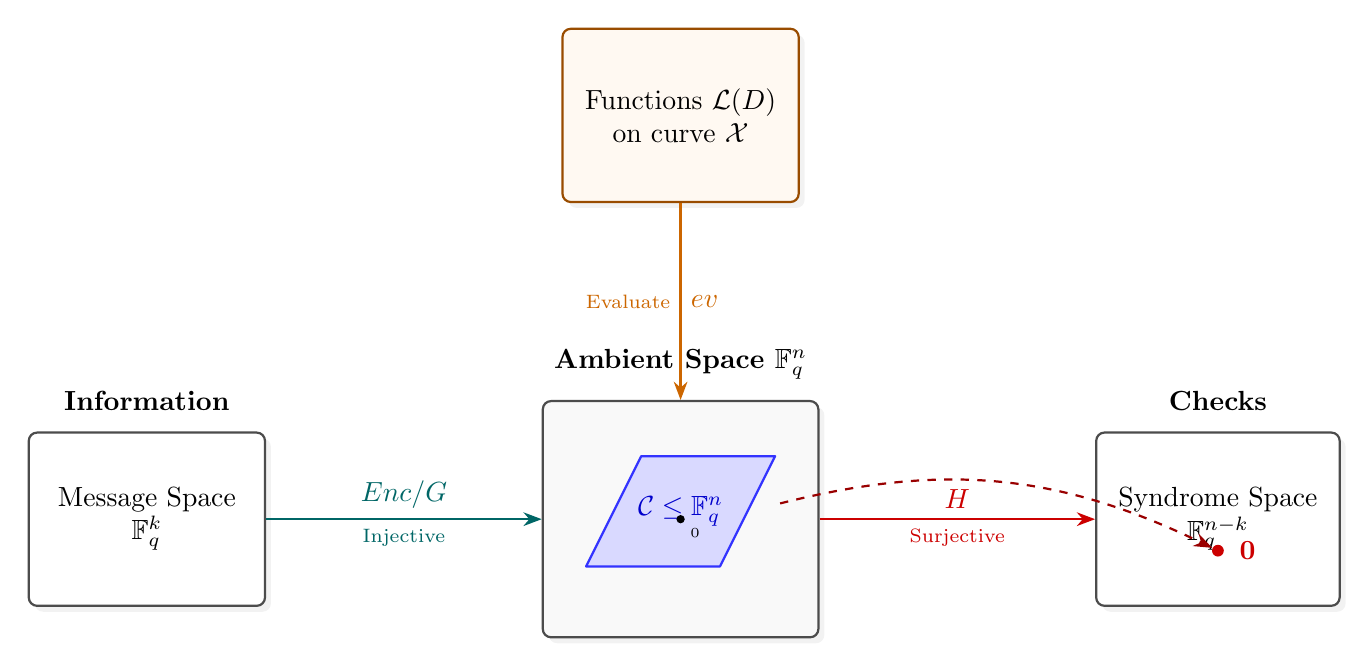
\begin{tikzpicture}[
			>=Stealth,
			spacebox/.style={
				draw=black!70, fill=white, thick, rounded corners=3pt, 
				inner sep=8pt, align=center, minimum height=2.2cm, minimum width=3cm,
				drop shadow={opacity=0.1}
			},
			matstyle/.style={font=\small, align=center}
			]
			
			% 1. AMBIENT SPACE & SUBSPACE (Center)
			\node[spacebox, fill=gray!5, minimum height=3cm, minimum width=3.5cm] (ambient) at (0,0) {};
			\draw[thick, fill=blue!15, draw=blue!80, join=round] 
			(-1.2,-0.6) -- (0.5,-0.6) -- (1.2,0.8) -- (-0.5,0.8) -- cycle;
			\node[font=\bfseries, text=blue!80!black] at (0,0.1) {$\C \leq \F_q^n$};
			\fill[black] (0,0) circle (1.5pt) node[below right, font=\tiny] {$0$};
			\node[above=4pt of ambient, font=\bfseries] {Ambient Space $\F_q^n$};
			
			% 2. MESSAGE SPACE & ENCODING (Left)
			\node[spacebox, left=3.5cm of ambient] (msg) {Message Space \\ $\F_q^k$};
			\draw[->, thick, teal!80!black] (msg.east) -- (ambient.west) 
			node[midway, above, font=\bfseries] {$Enc / G$} 
			node[midway, below, font=\scriptsize] {Injective};
			\node[above=4pt of msg, font=\bfseries] {Information};
			
			% 3. SYNDROME SPACE & PARITY CHECK (Right)
			\node[spacebox, right=3.5cm of ambient] (synd) {Syndrome Space \\ $\F_q^{n-k}$};
			\draw[->, thick, red!80!black] (ambient.east) -- (synd.west) 
			node[midway, above, font=\bfseries] {$H$} 
			node[midway, below, font=\scriptsize] {Surjective};
			\node[above=4pt of synd, font=\bfseries] {Checks};
			
			\node[circle, fill=red!80!black, inner sep=1.5pt] (zero) at ($(synd) + (0,-0.4)$) {};
			\node[right=2pt of zero, text=red!80!black, font=\bfseries] {$\mathbf{0}$};
			\draw[->, dashed, thick, red!60!black] ($(ambient.east) + (-0.5, 0.2)$) to[bend left=20] (zero);
			
			% 4. AG VIEWPOINT (Top)
			\node[spacebox, fill=orange!5, draw=orange!60!black, above=2.5cm of ambient] (ag) {
				Functions $\cL(D)$ \\ on curve $\X$
			};
			\draw[->, thick, orange!80!black] (ag.south) -- (ambient.north) 
			node[midway, right, font=\bfseries] {$ev$} 
			node[midway, left, font=\scriptsize] {Evaluate};
		\end{tikzpicture}
		\caption{The Structural Viewpoints of Block Codes.}
	\end{figure}
	
	\section{The Algebraic Foundation: Linear Subspaces}
	
	\begin{definition}
		Let $\Sigma = \F_q$ be a finite field. A \textbf{linear block code} $\C$ of length $n$ and dimension $k$ is a $k$-dimensional subspace of the ambient vector space $\F_q^n$. We denote this by $\C \leq \F_q^n$.
	\end{definition}
	
	By requiring $\C$ to be a linear subspace, it is closed under vector addition and scalar multiplication. The size of the code is exactly $|\C| = q^k$.
	
	\section{The Generative Viewpoint: Image of Encoding}
	
	To transmit information, we map raw $k$-dimensional messages into the $n$-dimensional ambient space.
	
	\begin{definition}
		The code $\C$ is the \textbf{image} of an injective linear map $Enc: \F_q^k \to \F_q^n$. This mapping is represented by a $k \times n$ full-rank \textbf{generator matrix} $G$.
		$$ \C = \text{Im}(G) = \{ mG \mid m \in \F_q^k \} $$
	\end{definition}
	
	The rows of $G$ form a basis for the linear subspace $\C$.
	
	\section{The Checking Viewpoint: Kernel of Parity}
	
	Alternatively, a subspace can be defined by the linear constraints its elements must satisfy.
	
	\begin{definition}
		The code $\C$ is the \textbf{kernel} of a surjective linear map $H: \F_q^n \to \F_q^{n-k}$, represented by an $(n-k) \times n$ full-rank \textbf{parity-check matrix} $H$.
		$$ \C = \text{Ker}(H) = \{ c \in \F_q^n \mid Hc^T = \mathbf{0} \} $$
	\end{definition}
	
	This requires that the row space of $G$ and the row space of $H$ are orthogonal complements, meaning $GH^T = \mathbf{0}$. Together, these define the fundamental exact sequence of linear coding theory:
	$$ 0 \to \F_q^k \xrightarrow{G} \F_q^n \xrightarrow{H} \F_q^{n-k} \to 0 $$
	
	\section{The Algebraic Geometry (AG) Viewpoint}
	
	The AG viewpoint provides a powerful way to construct the subspace $\C$ not via matrices, but by evaluating functions on algebraic curves. 
	
	Let $\X$ be a smooth, projective algebraic curve of genus $g$ defined over $\F_q$. Let $P_1, P_2, \dots, P_n$ be distinct $\F_q$-rational points on $\X$. Let $D$ be a divisor on $\X$ whose support is disjoint from $\{P_1, \dots, P_n\}$.
	
	\begin{definition}
		The \textbf{Riemann-Roch space} associated with $D$ is:
		$$ \cL(D) = \{ f \in \F_q(\X)^* \mid (f) + D \geq 0 \} \cup \{0\} $$
	\end{definition}
	This space consists of rational functions whose poles are constrained by the divisor $D$. It is a finite-dimensional vector space over $\F_q$.
	
	We define the evaluation map $ev: \cL(D) \to \F_q^n$ by:
	$$ ev(f) = (f(P_1), f(P_2), \dots, f(P_n)) $$
	
	The \textbf{Algebraic Geometry Code} $\C(D, P_1\dots P_n)$ is the image of this map.
	
	\subsection{Dimension and the Riemann-Roch Theorem}
	
	To find the dimension $k$ of our code $\C$, we must determine the dimension of the function space $\cL(D)$, denoted $l(D)$. 
	\begin{theorem}[Riemann-Roch]
		For any divisor $D$ on a curve of genus $g$:
		$$ l(D) - l(K - D) = \deg(D) + 1 - g $$
		where $K$ is the canonical divisor.
	\end{theorem}
	
	If we choose $D$ such that $2g - 2 < \deg(D) < n$, the term $l(K-D) = 0$. Furthermore, the condition $\deg(D) < n$ guarantees that a non-zero function cannot have $n$ roots, making the evaluation map $ev$ strictly injective. Therefore, the dimension of the code is exactly:
	$$ k = \deg(D) + 1 - g $$
	
	\begin{remark}
		The minimum distance $d$ of this code satisfies the Goppa bound: $d \geq n - \deg(D)$. This shows how choosing curves with many rational points relative to their genus allows AG codes to exceed classical bounds.
	\end{remark}
	
\end{document}